\documentclass[10pt, pdf, hyperref={unicode}]{beamer}
\usetheme{metropolis} 

\usepackage{polyglossia}
\setdefaultlanguage[spelling=modern]{russian}

\usepackage{caption}
\captionsetup[figure]{labelformat=empty, font=scriptsize}
\captionsetup[subfigure]{labelformat=empty, font=scriptsize}
\captionsetup[table]{labelformat=empty, font=scriptsize}

\usepackage{bibentry}
\nobibliography*

\setbeamercolor{background canvas}{bg=white}
%\setbeamerfont{bibliography item}{size=\tiny}
%\setbeamerfont{bibliography entry author}{size=\tiny}
%\setbeamerfont{bibliography entry title}{size=\tiny}
%\setbeamerfont{bibliography entry location}{size=\tiny}
%\setbeamerfont{bibliography entry note}{size=\tiny}

\usepackage{subcaption}

\title{Оптический отклик Ми-резонансных наночастиц, связанных с диэлектрическими волноводами}
\date{}
\author{Нестеров~К.\,Е.}
\institute{
	МОСКОВСКИЙ ГОСУДАРСТВЕННЫЙ УНИВЕРСИТЕТ имени М.В.ЛОМОНОСОВА \\
	ФИЗИЧЕСКИЙ ФАКУЛЬТЕТ МГУ \\
	Кафедра квантовой электроники
}

\begin{document}
  	\maketitle
  
  	\begin{frame}{Оптические метаматериалы}
    \begin{minipage}[b]{.5\textwidth}
    	Неметаллические
    	\begin{figure}
    		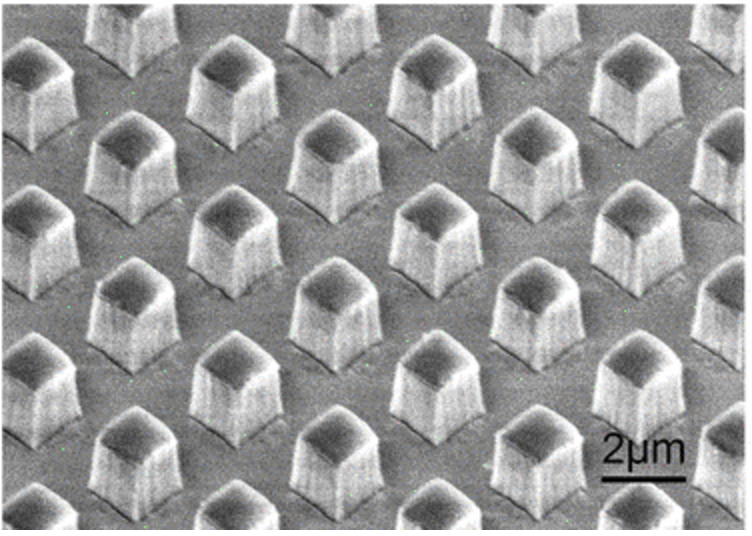
\includegraphics[width=\textwidth]{img/Ginn}
    		\caption{\bibentry{Ginn2012}}
    	\end{figure}
    \end{minipage}
\end{frame}
  	\begin{frame}{Рассеяние Ми}
	\begin{minipage}[t][\textheight]{.5\textwidth}
		\begin{figure}
			\centering
			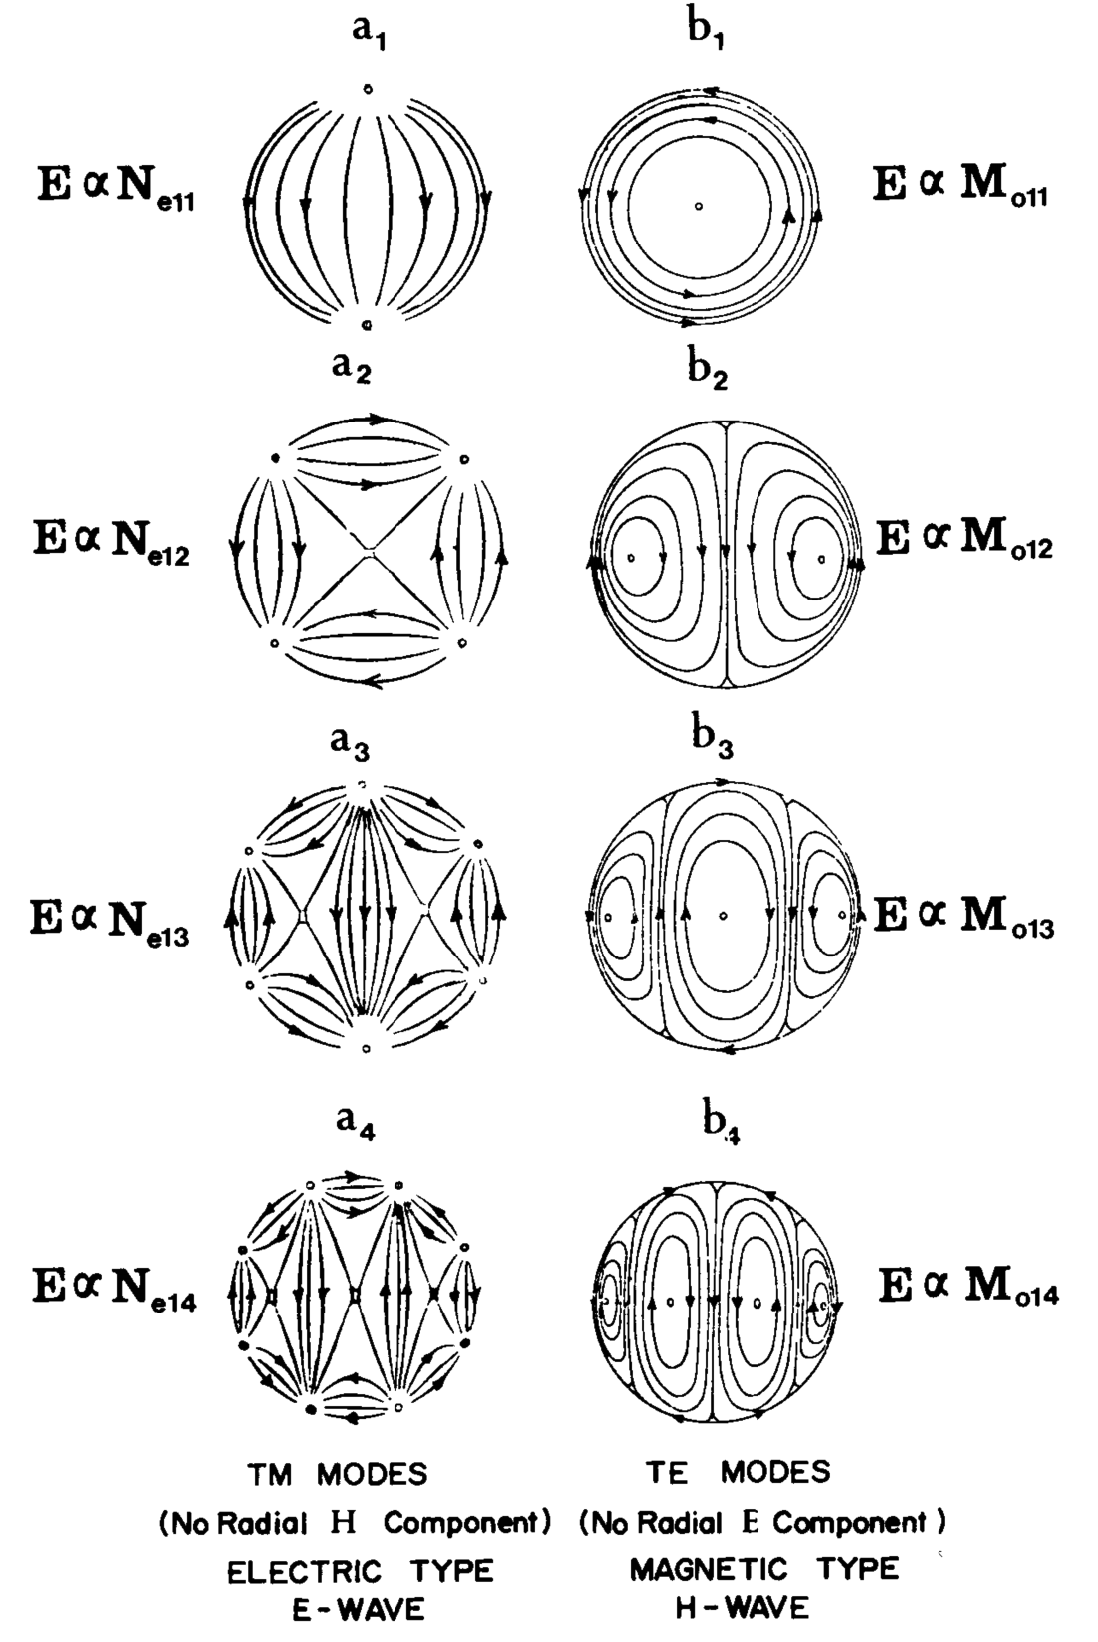
\includegraphics[width=.8\textwidth]{img/Mie_total}
			\caption{\bibentry{Bohren1998}}
		\end{figure}
	\end{minipage}%
	\begin{minipage}[t][\textheight]{.5\textwidth}
		\begin{figure}
			\centering
			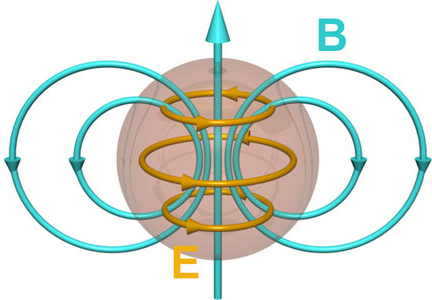
\includegraphics[width=\textwidth]{img/mie_reson}
			\caption{\bibentry{Kuznetsov2012}}
		\end{figure}

		\begin{itemize}
			\item Сферы, позже цилиндры
			\item Первая магнитная мода
			\item Ненулевой магнитный дипольный момент	
		\end{itemize}
	\end{minipage}
\end{frame}
  	\begin{frame}{Сверхбыстрые полностью оптические переключатели}
	\begin{figure}
		\begin{subfigure}{.35\textwidth}
			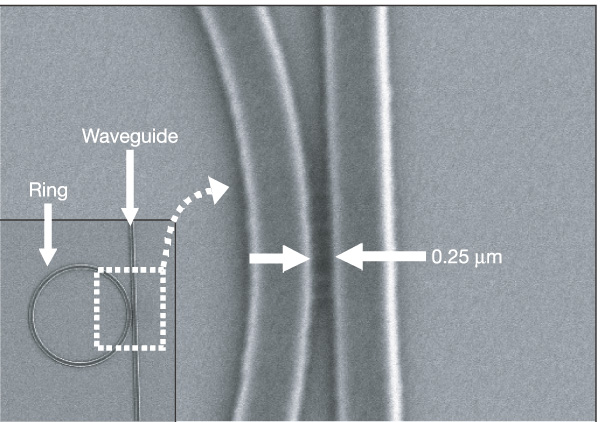
\includegraphics[width=.95\textwidth]{img/ring}
			\vspace{.5em}
			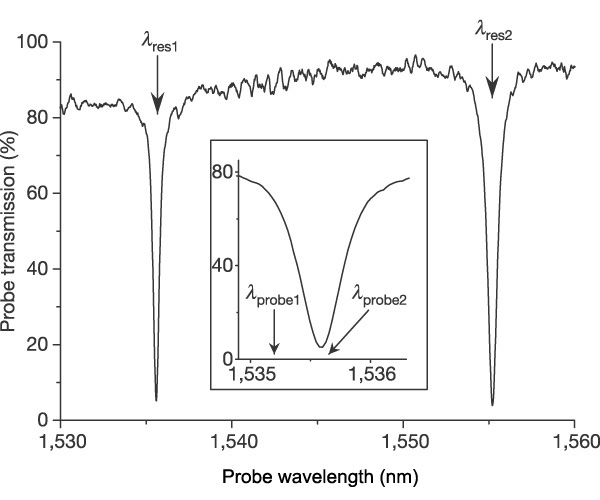
\includegraphics[width=.95\textwidth]{img/ring_spectrum}
		\end{subfigure}%
		\begin{subfigure}{.65\textwidth}
			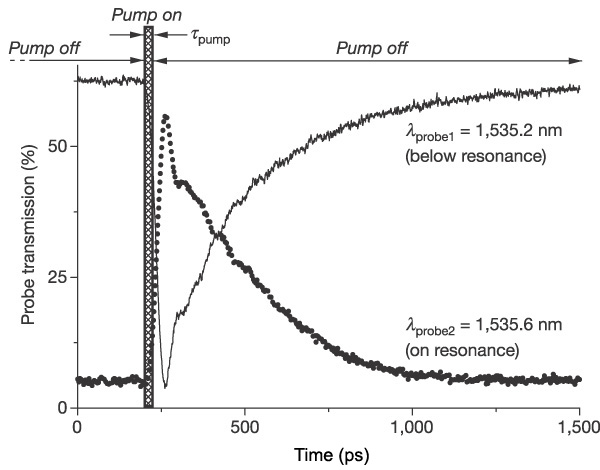
\includegraphics[width=\textwidth]{img/ring_res_shift}
		\end{subfigure}
		\caption{\bibentry{Vilson2004}}
	\end{figure}%
	\begin{itemize}
		\item Изменение показателя преломления путём двухфотонного поглощения
	\end{itemize}
\end{frame}
  	\begin{frame}{Исследуемые наноструктуры}
	\begin{minipage}[b]{.5\textwidth}
		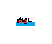
\includegraphics[width=.95\textwidth]{img/scheme_yz3}
		
		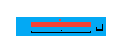
\includegraphics[width=.9\textwidth]{img/scheme_xy3}
		\vspace{3em}
	\end{minipage}%
	\begin{minipage}[b]{.5\textwidth}
		\begin{table}
			\begin{tabular}{|c|c|}
				\hline
				Параметр & Значение\\
				\hline
				\hline
				$\lambda$ & 1.0 мкм--2.0 мкм \\
				\hline
				$L$ & 10 мкм \\
				\hline
				$w$ & 0.6 мкм \\
				\hline
				$h$ & 0.25 мкм, 0.4 мкм \\
				\hline
				$r$ & 0.1 мкм--1.0 мкм\\
				\hline
				$d$ & $-$0.09 мкм--1.0 мкм\\
				\hline
				$N$ & 1--20 \\
				\hline
				$D_{i, i+1}$ & 0 мкм--0.4 мкм \\
				\hline
			\end{tabular}
		\end{table}
	\end{minipage}
	
	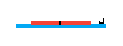
\includegraphics[width=\textwidth]{img/scheme_xz}
\end{frame}
  	\begin{frame}{Система волновод\,--\,нанодиск}
	\begin{minipage}{.8\textwidth}
		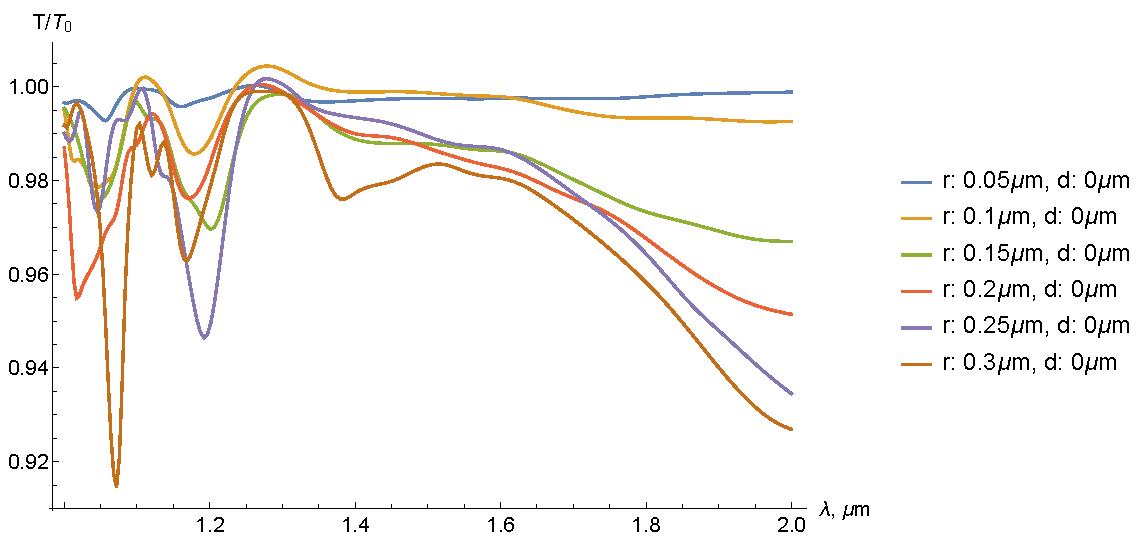
\includegraphics[width=\textwidth]{img/total_d0_theta_0}
	
		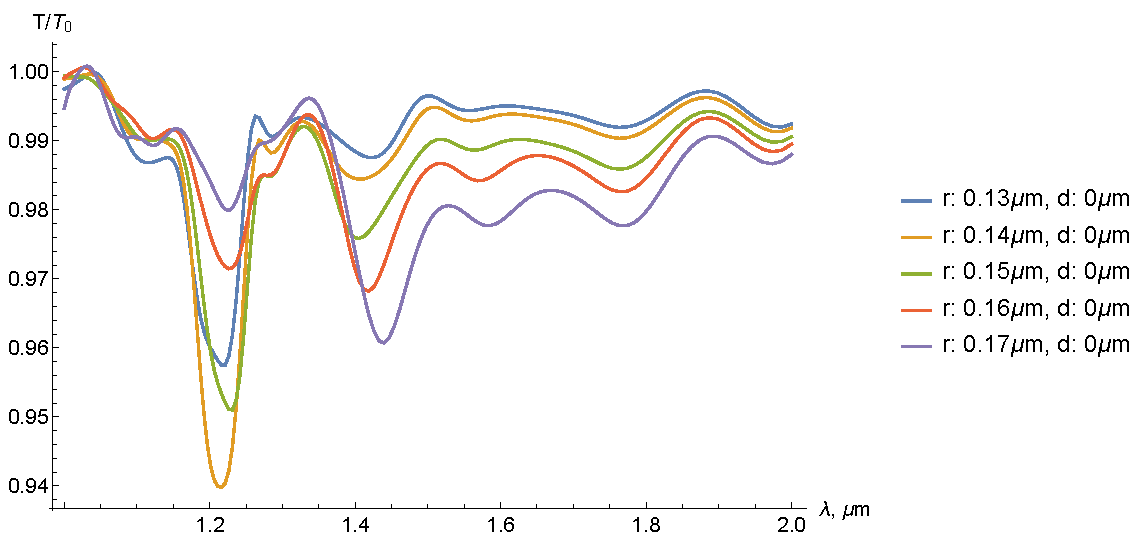
\includegraphics[width=\textwidth]{img/total_d0_theta_90-short}	
	\end{minipage}%
	\begin{minipage}{.2\textwidth}
		$$E_{\parallel}$$
		\vspace{6em}
		$$E_{\bot}$$
	\end{minipage}

\end{frame}

\begin{frame}{Система волновод\,--\,нанодиск}
	\centering
	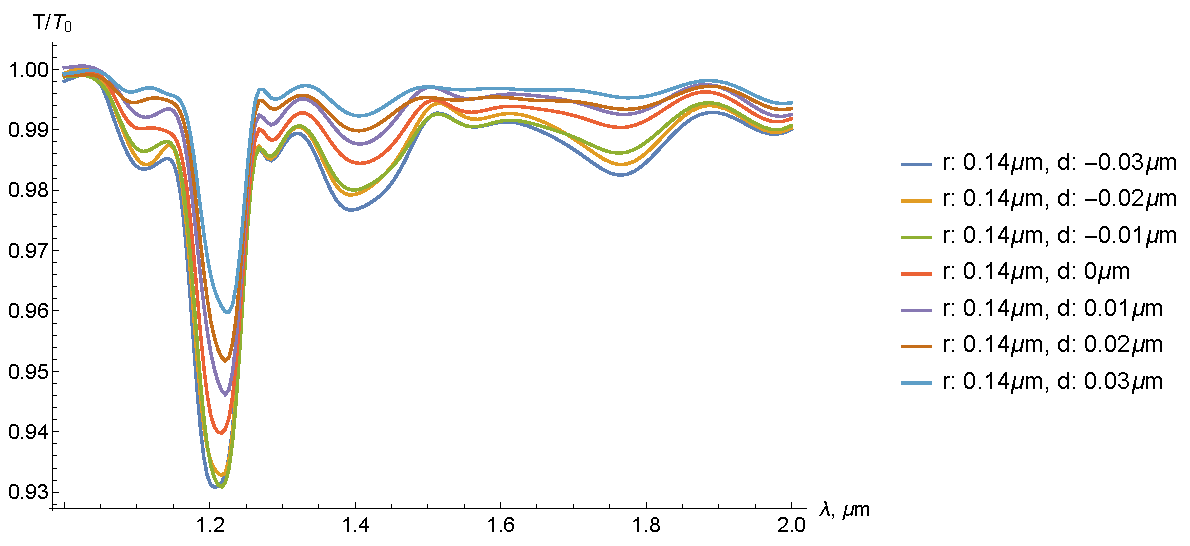
\includegraphics[width=\textwidth]{img/r_014_d_var}
	
	\begin{figure}
		\begin{subfigure}[b]{.5\textwidth}
			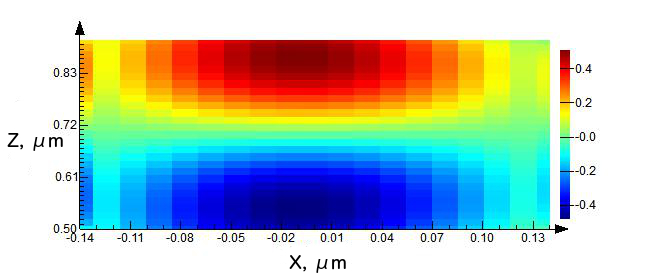
\includegraphics[width=\textwidth]{img/E_x_014_presentation}
			\caption{$E_x$}
		\end{subfigure}%
		\begin{subfigure}[b]{.5\textwidth}
			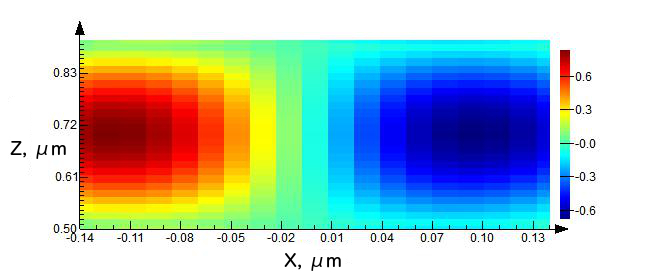
\includegraphics[width=\textwidth]{img/E_z_014_presentation}
			\caption{$E_z$}
		\end{subfigure}
	\end{figure}
\end{frame}
  	\begin{frame}{Система волновод\,--\,массив нанодисков}
	\begin{figure}[h]
		\centering
		\begin{subfigure}[b]{.7\textwidth}
			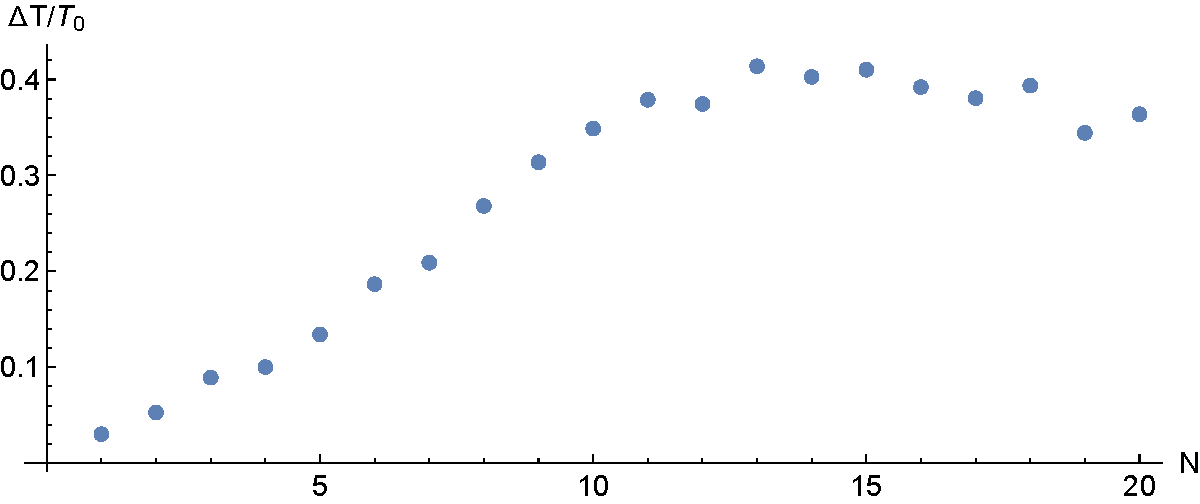
\includegraphics[width=\textwidth]{img/dTPlot-presentation}
			\caption{Глубина пика}
			\label{fig:metrics_dT}
		\end{subfigure}
		\begin{subfigure}[b]{.75\textwidth}
			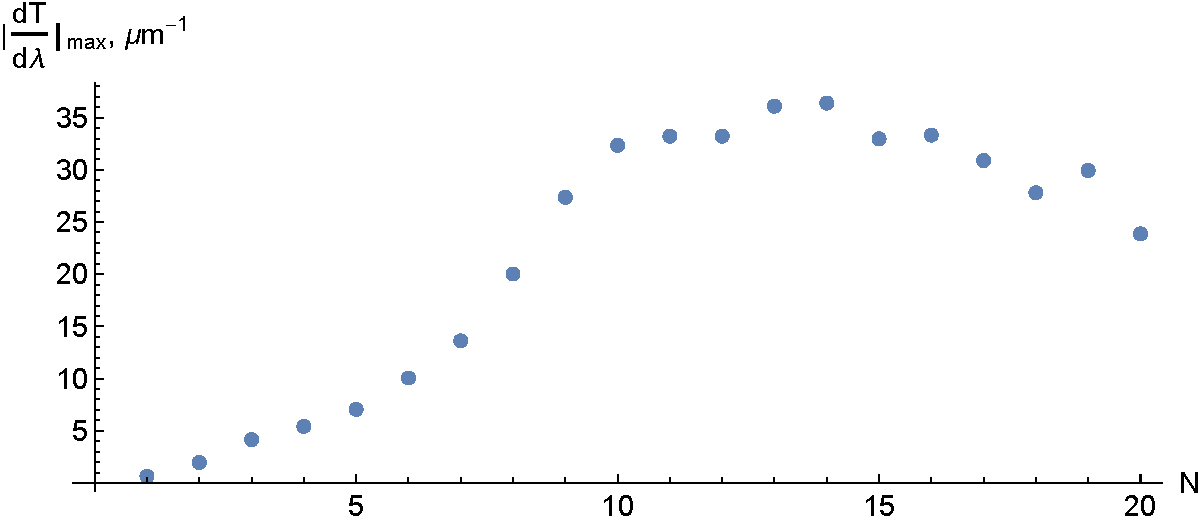
\includegraphics[width=\textwidth]{img/dTdλPlot-presentation}
			\caption{''Острота`` резонанса}
			\label{fig:metrics_dTdLambda}
		\end{subfigure}
	\end{figure}
\end{frame}
\begin{frame}{Система волновод\,--\,массив нанодисков}
	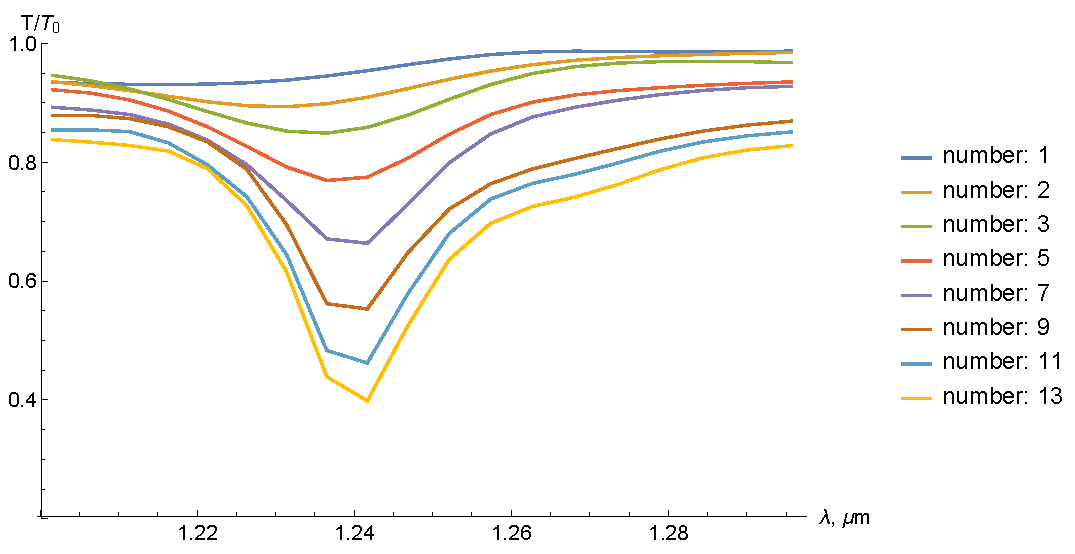
\includegraphics[width=\textwidth]{img/total}
	
	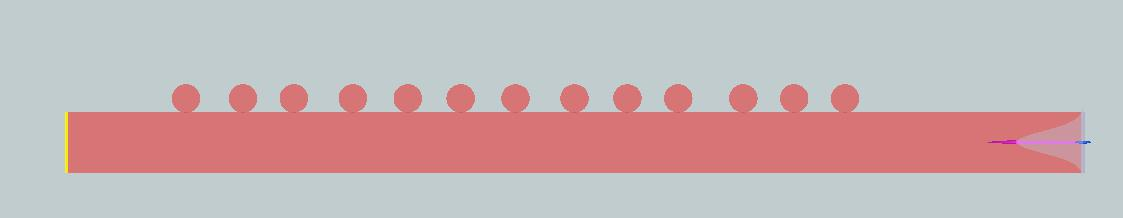
\includegraphics[width=\textwidth]{img/view_xy_13}
\end{frame}
  	\begin{frame}{Сравнение с функциональными аналогами}
	Важны площадь структуры, время отклика и максимальная производная пика
	\begin{table}
		\centering
		\begin{tabular}{|c|c|c|}
			\hline
			Сравниваемая структура & $\left(dT/d\lambda\right)_{max}/S$, $\mu m^{-3}$ & 	$1/\Delta \omega$, с \\
			\hline
			Одиночный нанодиск & $19.7$ & $7.8 \cdot 10^{-14}$\\
			\hline
			Массив нанодисков & $19.1$ & $2.8 \cdot 10^{-13}$\\
			\hline
			Кольцевой резонатор ($Si$) \footnotemark & $1.3 \cdot 10^3$ & $1.5 \cdot 10^{-11}$\\
			\hline
			Кольцевой резонатор ($Si_3 N_4$) \footnotemark & $3 \cdot 10^3$ & $1.5 \cdot 10^{-8}$\\
			\hline
			Дисковый резонатор ($Si$) \footnotemark & $6.7 \cdot 10^2$ & $1.0 	\cdot 10^{-8}$\\
			\hline
		\end{tabular}
	\end{table}
	
	\footnotetext[1]{\bibentry{Vilson2004}}
	\footnotetext[2]{\bibentry{Gondarenko2009}}
	\footnotetext[3]{\bibentry{Soltani2007}}
\end{frame}
  	\begin{frame}{Выводы}
	\begin{itemize}
		\item Численно определены оптимальные параметры системы из одного нанодиска, связанного с волноводом, для эффективного возбуждения магнитного резонанса.
		\item Последовательно численно определены оптимальные параметры системы из нескольких связанных с волноводом нанодисков в зависимости от их количества.
		\item Рассмотрены как системы с односторонним, так и с двухсторонним расположением дисков относительно волновода.
		\item Обнаружен ''эффект насыщения`` резонанса от количества резонаторов и определены предельные характеристики, достижимые на подобной конфигурации.
		\item Введена метрика и проведено сравнение с существующими решениями, близкими по функциональности. 
	\end{itemize}
\end{frame}
  
  	\begin{frame}
  		\bibliographystyle{presentation}
		\bibliography{literature-abbrv}
  	\end{frame}
\end{document}